\documentclass{article}

\usepackage[pdftex]{graphicx}
\graphicspath{{img/}}

\usepackage{hyperref}
\usepackage{url} \urlstyle{sf}

\usepackage{color}
\def\todo#1{{\color{red}TODO\@: #1}}
\def\addref#1{{\color{red}$[$#1$]$}}

\usepackage{fullpage}
\usepackage{float}
\usepackage{amssymb}

\title{Exact Analysis of the Cache Behavior of Nested Loops\\
        \large Critical Synthesis}

\author{Simon Bihel}

% ought to be 3-5 pages
% the presentation ought to be 20 minutes long
\begin{document}
\maketitle

\section{Introduction}
This is a synthesis of~\cite{chatterjee2001exact}.

In order to optimize a program you need to measure or predict its performances.
A simple method is to execute it or simulate the execution of the program to measure the performances, but this has the drawback of being highly computational.
The authors of the paper propose an exact model of the cache behavior of loop nests to make it possible to compute the exact performances of the cache as you could do with a simulation, but faster and with more insights on the behavior.

In Section~\ref{context} we explain the problem the authors aim to solve along with the tool they use.
After that in Section~\ref{model} we see how they employ these tools to effectively model the cache behavior of loop nests.
Section~\ref{eval} presents the evaluation of the contribution.
Section~\ref{critic} sums up the contribution in the light of a more critical point-of-view.

\section{Context}
\label{context}

\subsection{Memory Hierarchies}
The memory hierarchy considered is a simplified one, with one memory access at a time, no distinction between reads and writes, composed of two levels, and with a Least Recently Used replacement policy.

The goal is to count cache hits and misses.
The authors differentiate two kinds of misses.
\begin{description}
        \item[Interior misses] are misses that are independent of the initial cache state when the program fragment starts its execution.
        \item[Boundary misses] are misses that depend on the initial cache state.
\end{description}
In other words there are three kinds of memory accesses: those that are guaranteed to hit, those that are guaranteed to miss, and those that could hit or miss depending on the cache initial state.

\subsection{Polyhedral Model}
\begin{figure}
        \centering
        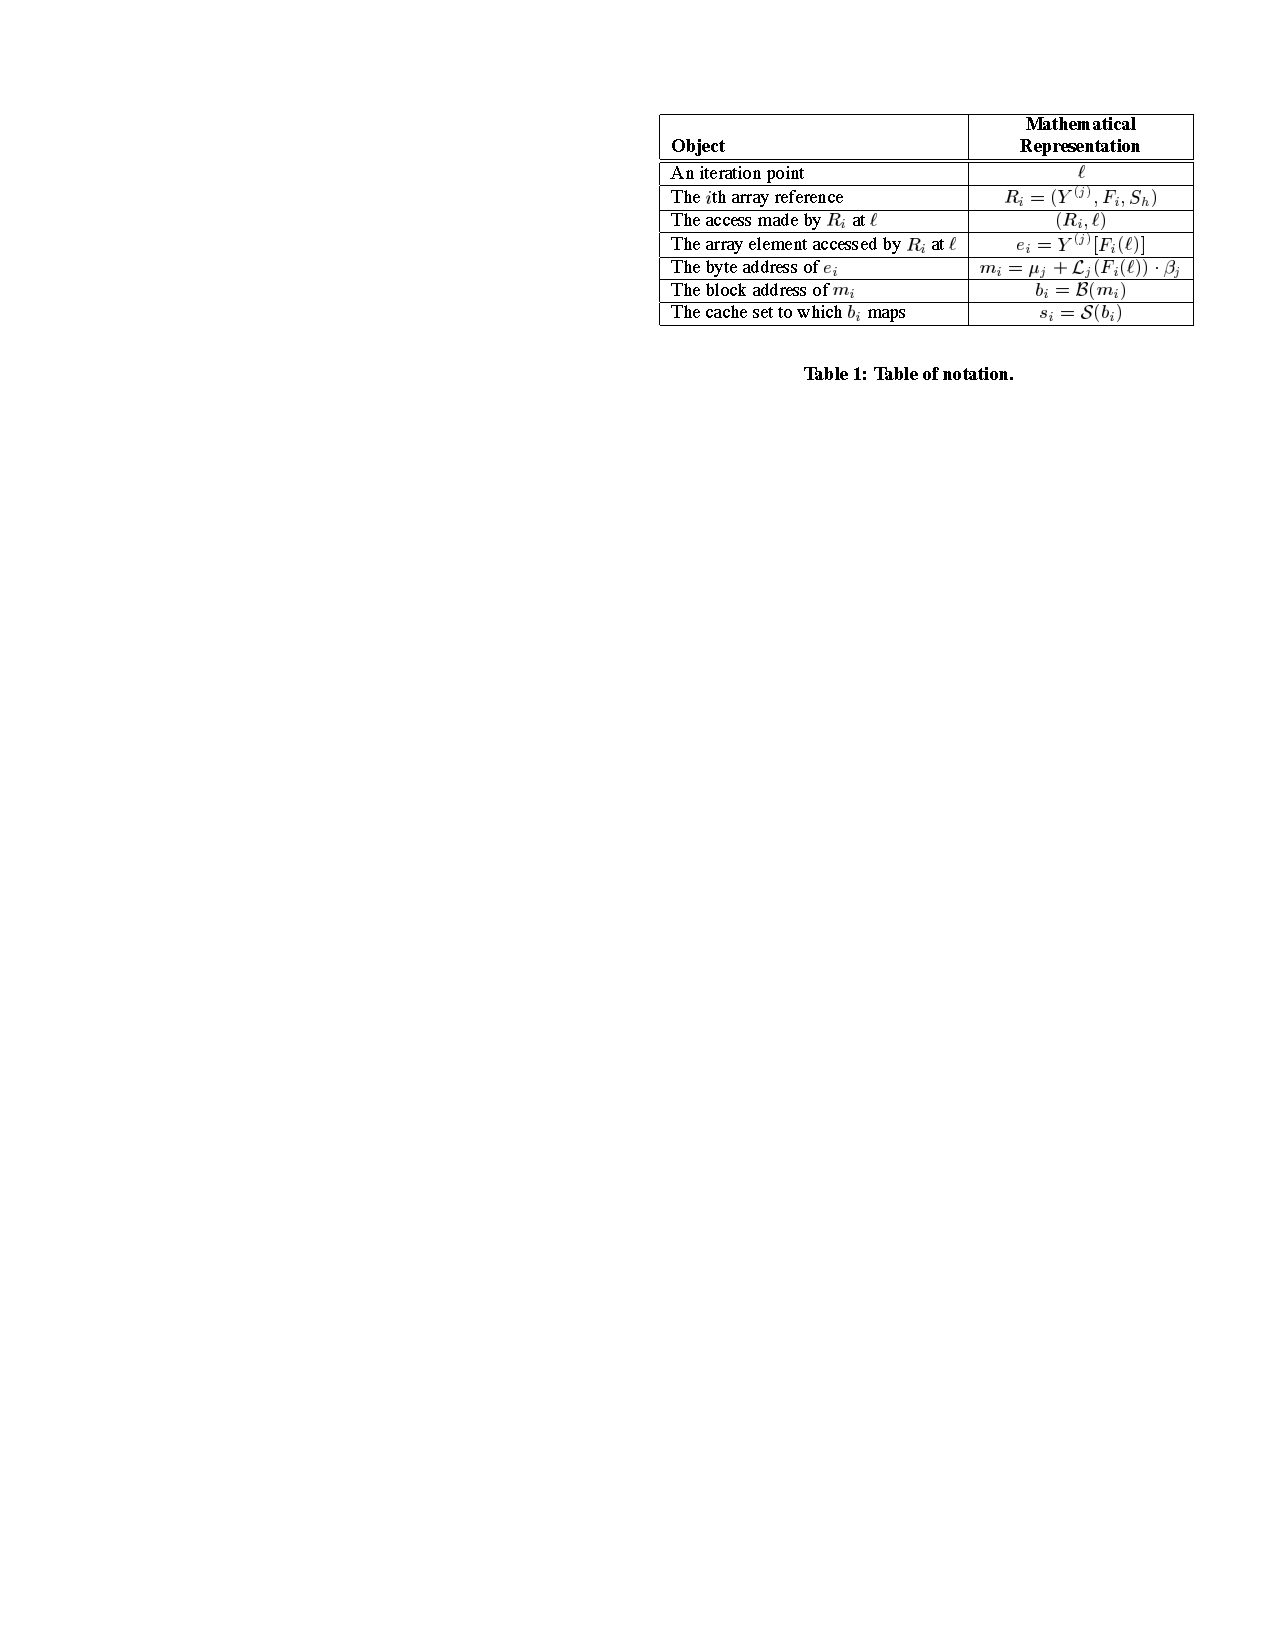
\includegraphics[trim={0 0.6cm 0 0}, clip, scale=1.1]{table1}
        \caption{Table of notation}
\label{fig:table1}
\end{figure}

Loop nests can be described mathematically.
\figurename~\ref{fig:table1} sums up the notations used for the polyhedral model.
An iteration point is an array of indexes to express the position in each loop.

More details will be given when needed when describing the model in Section~\ref{model}.

\subsection{Presburger Arithmetic}

Presburger arithmetic is a subset of first order logic consisting of constraints (equality or inequality) on integer variables.
The logical operators available are $\neg$, $\wedge$ and $\vee$, and the quantifiers available are $\forall$ and $\exists$.
With such formulas it is possible to describe cache structure and accesses, and thus compute misses.


\section{Cache Analysis Model}
\label{model}
In this section only a few formulas are presented by a lack of space.

\subsection{Cache Structure}

\subsubsection{Valid iteration point}
The first basic formula (1) is to describe an iteration point.
$d$ is the number of levels of nesting and $\ell_i$ the current index for the $i$-th loop.
That index has to be valid, i.e.\ in the index range ($0$ to $n_i$).
\begin{figure}[H]
        \centering
        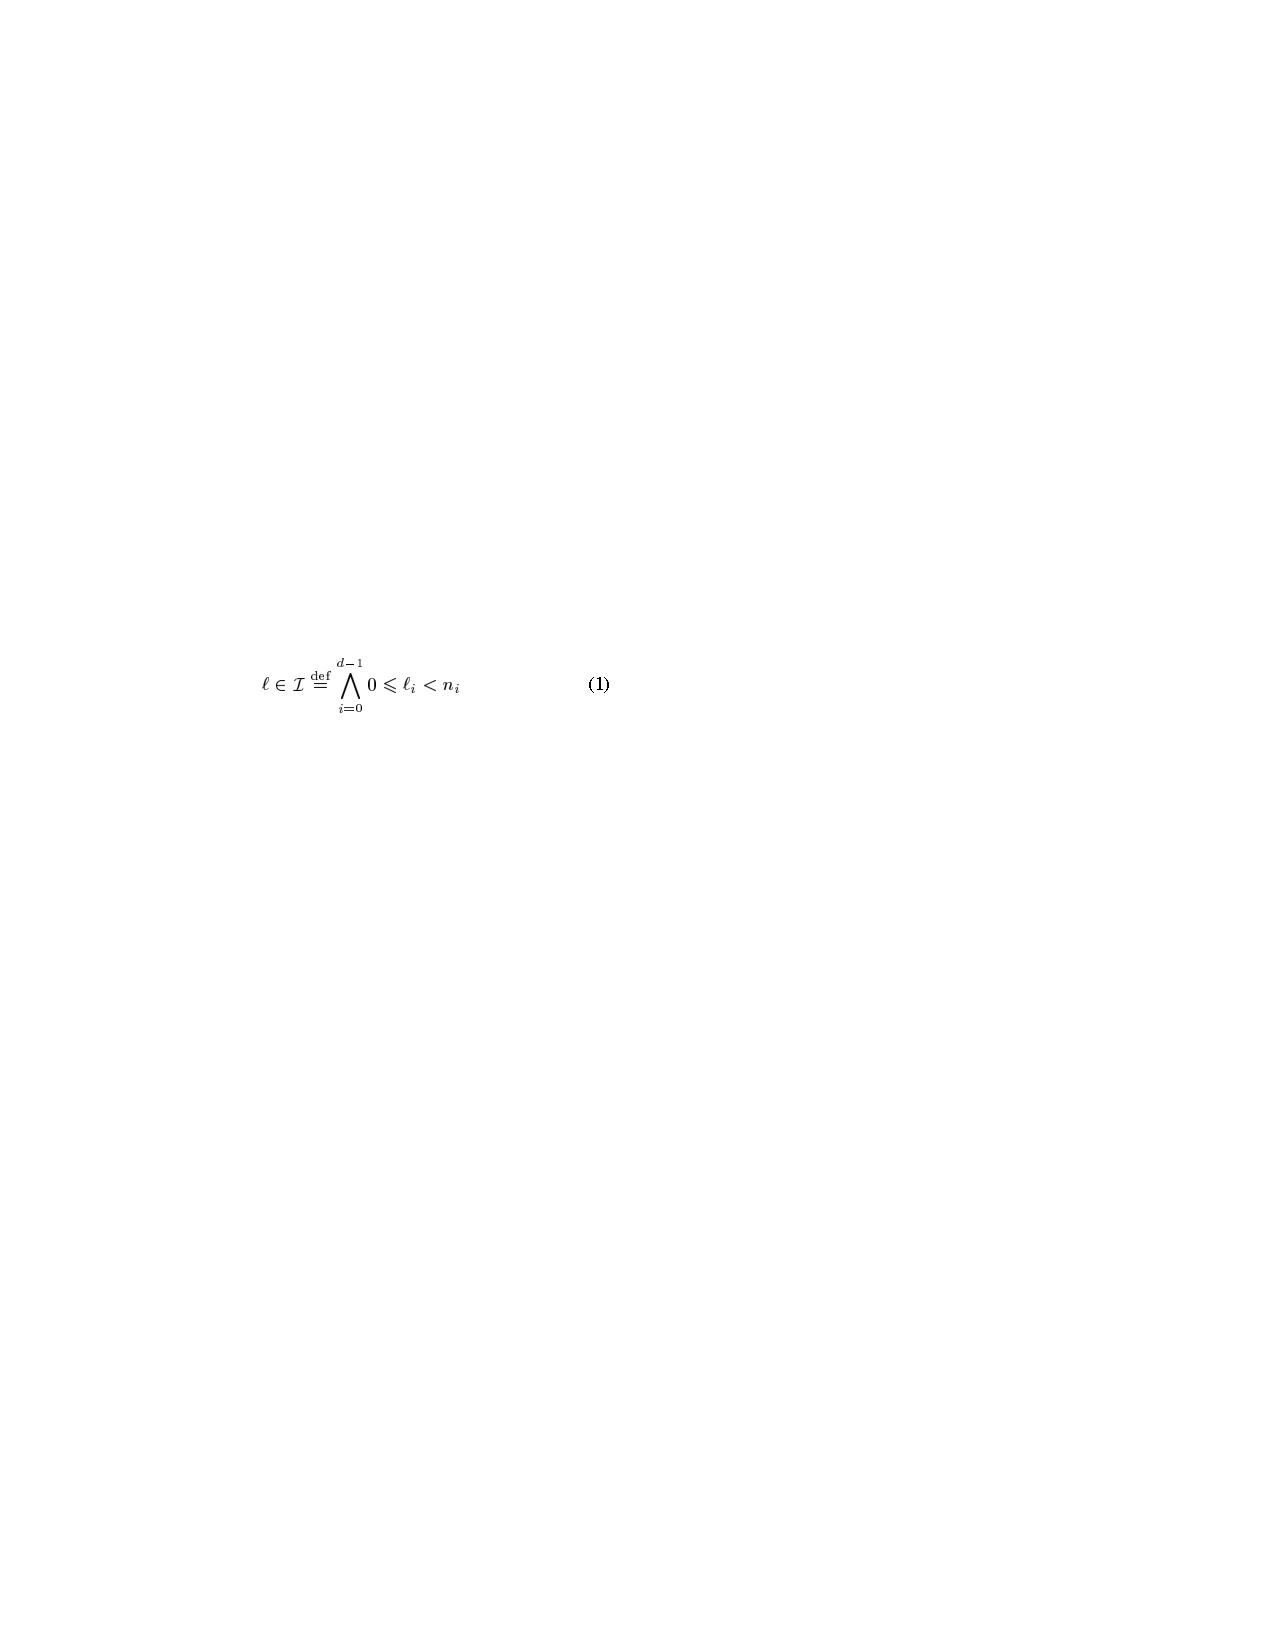
\includegraphics[scale=1.1]{eq1}
\label{fig:eq1}
\end{figure}


\subsubsection{Lexicographical ordering of accesses}
Then we need to express order in access.
Formula (2) describes that for iteration points $l$ and $m$, and for references $R_u$ and $R_v$.
It means that if $l$ is an iteration point that precedes $m$ then the references are obviously preceding, but if $l = m$ then we need to make sure $R_u$ occurs before $R_v$. % (comparison of the index expressions $F_u$ and $F_v$).
\begin{figure}[H]
        \centering
        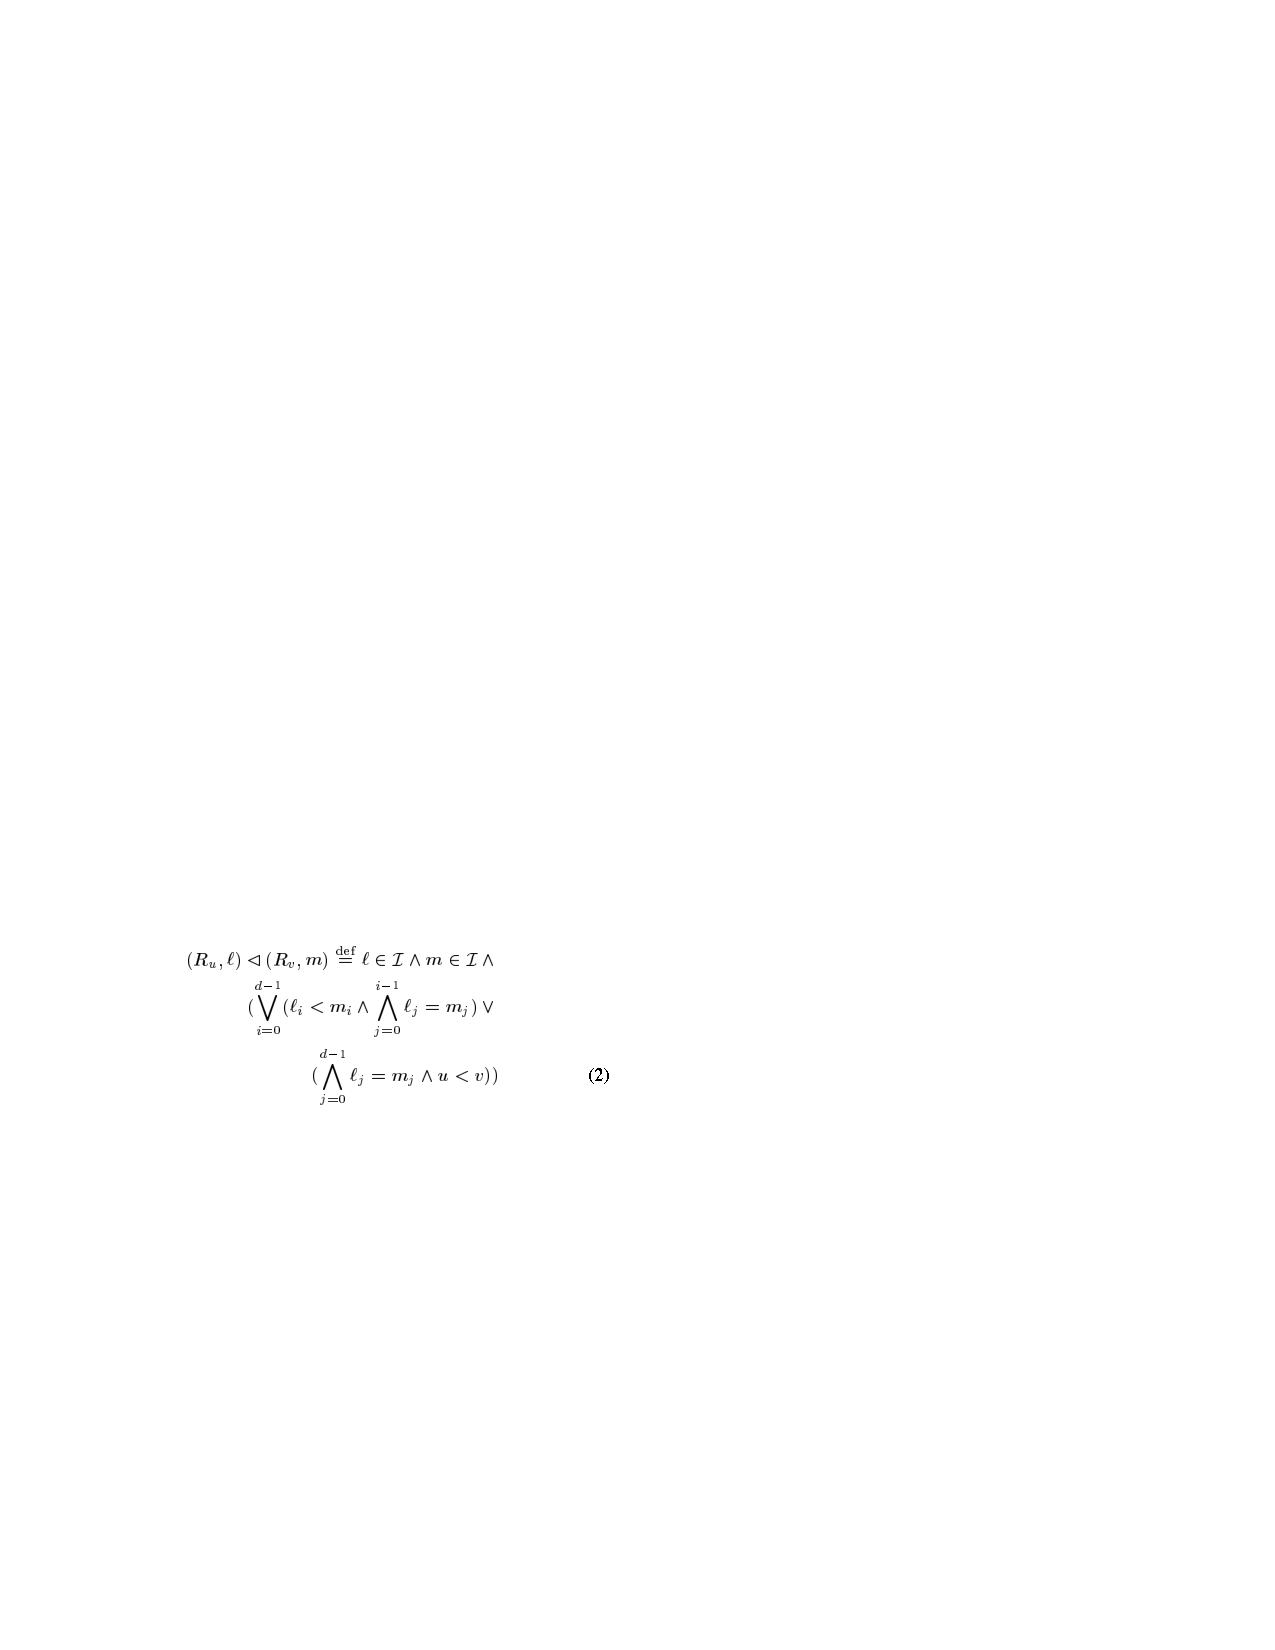
\includegraphics[scale=1.1]{eq2}
\label{fig:eq2}
\end{figure}

\subsubsection{Mapping memory locations to cache sets}
% \begin{figure}[H]
%         \centering
%         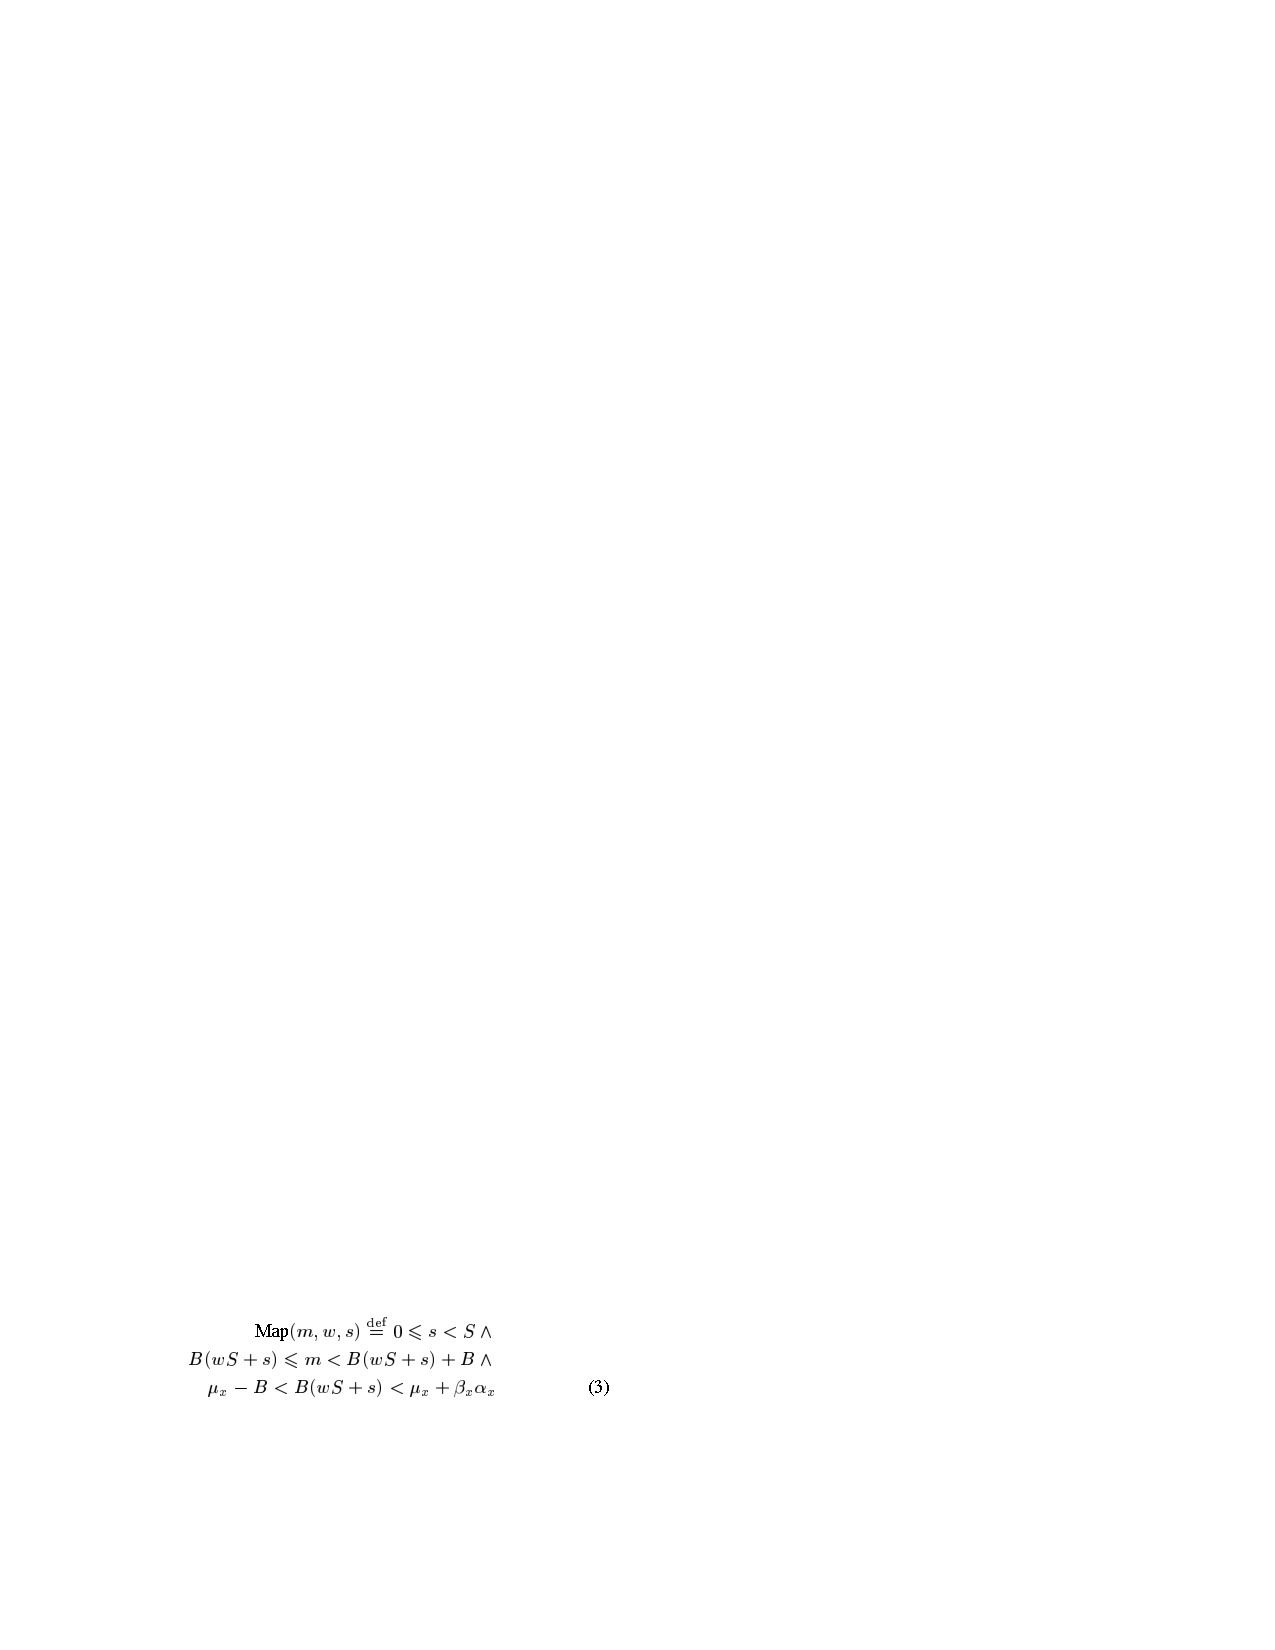
\includegraphics[scale=1.1]{eq3}
% \label{fig:eq3}
% \end{figure}
To express the memory location mapping to a cache set, they bound the memory value with cache sets boundaries while making sure it falls on a valid memory block boundary.

% \subsubsection{Data layouts in memory}
% % \begin{figure}[H]
% %         \centering
% %         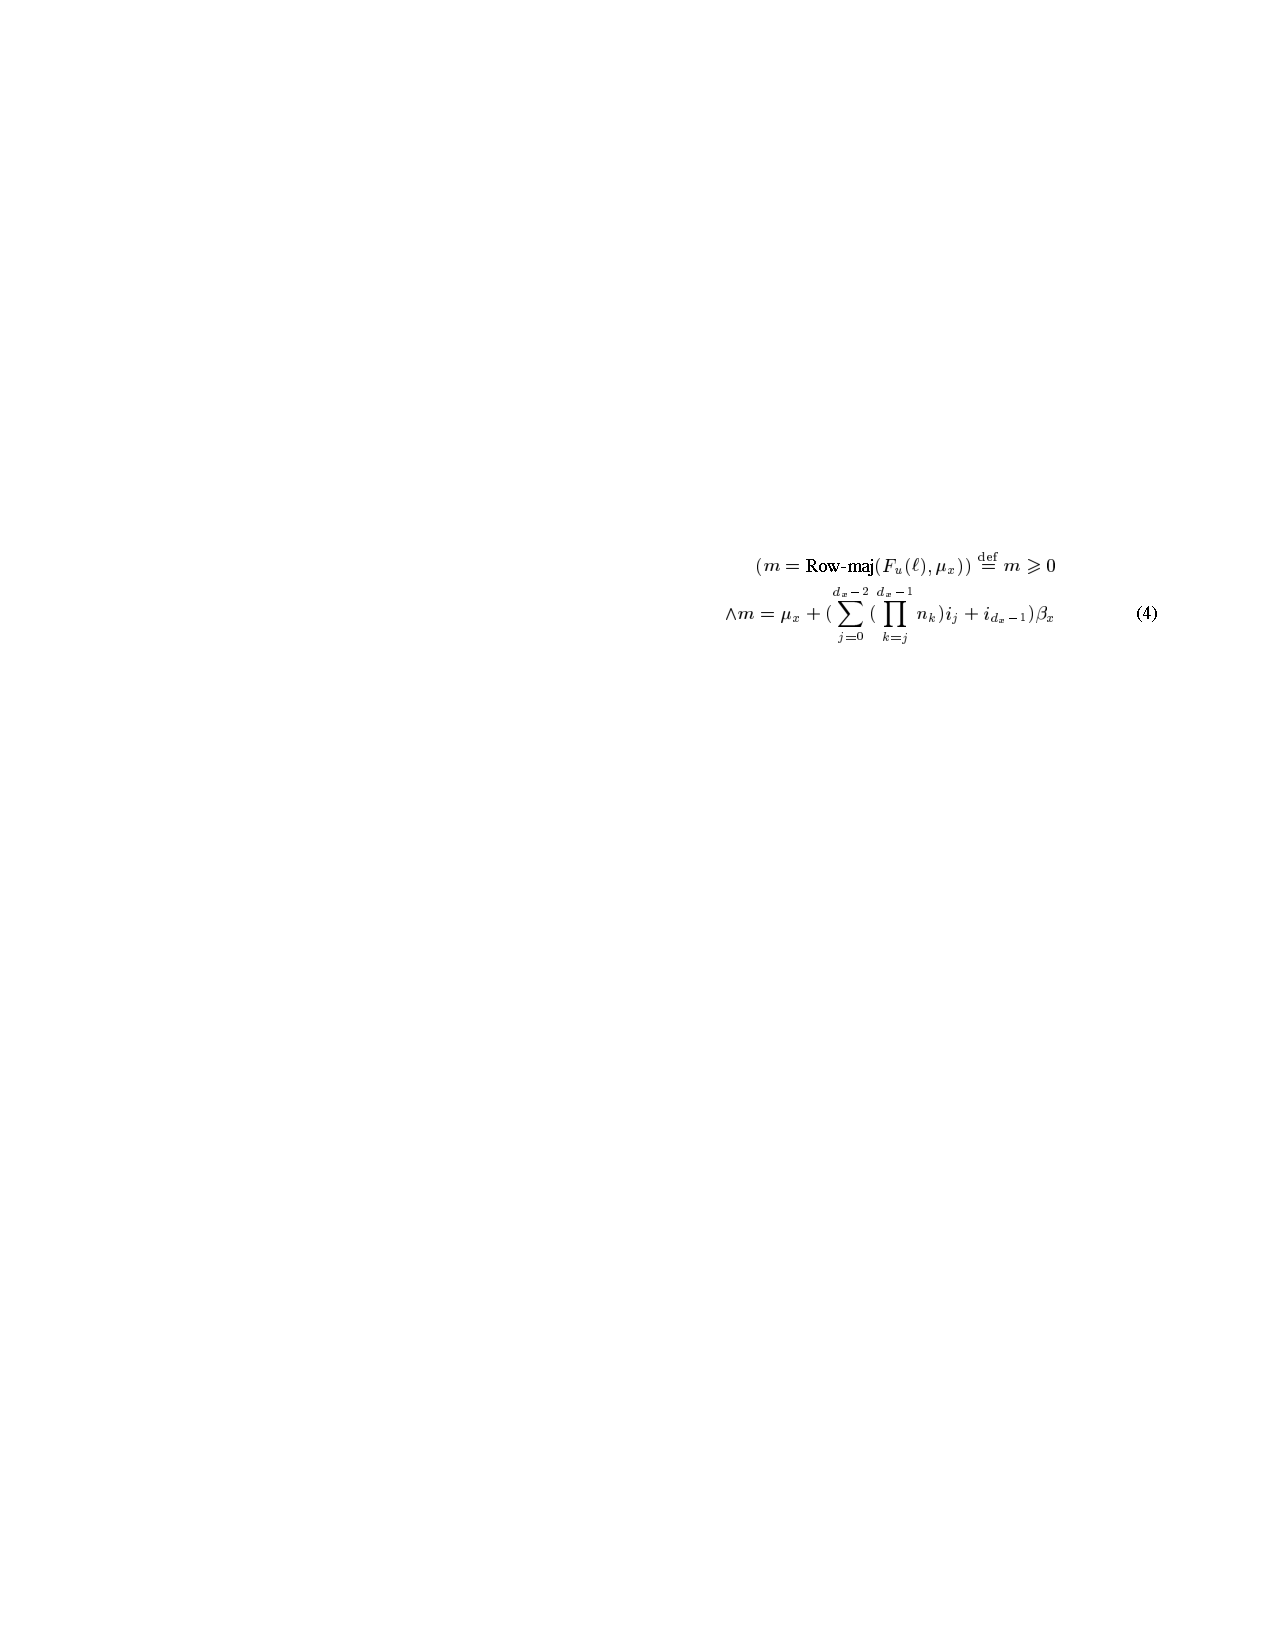
\includegraphics[scale=1.1]{eq4}
% % \label{fig:eq4}
% % \end{figure}
% % \begin{figure}[H]
% %         \centering
% %         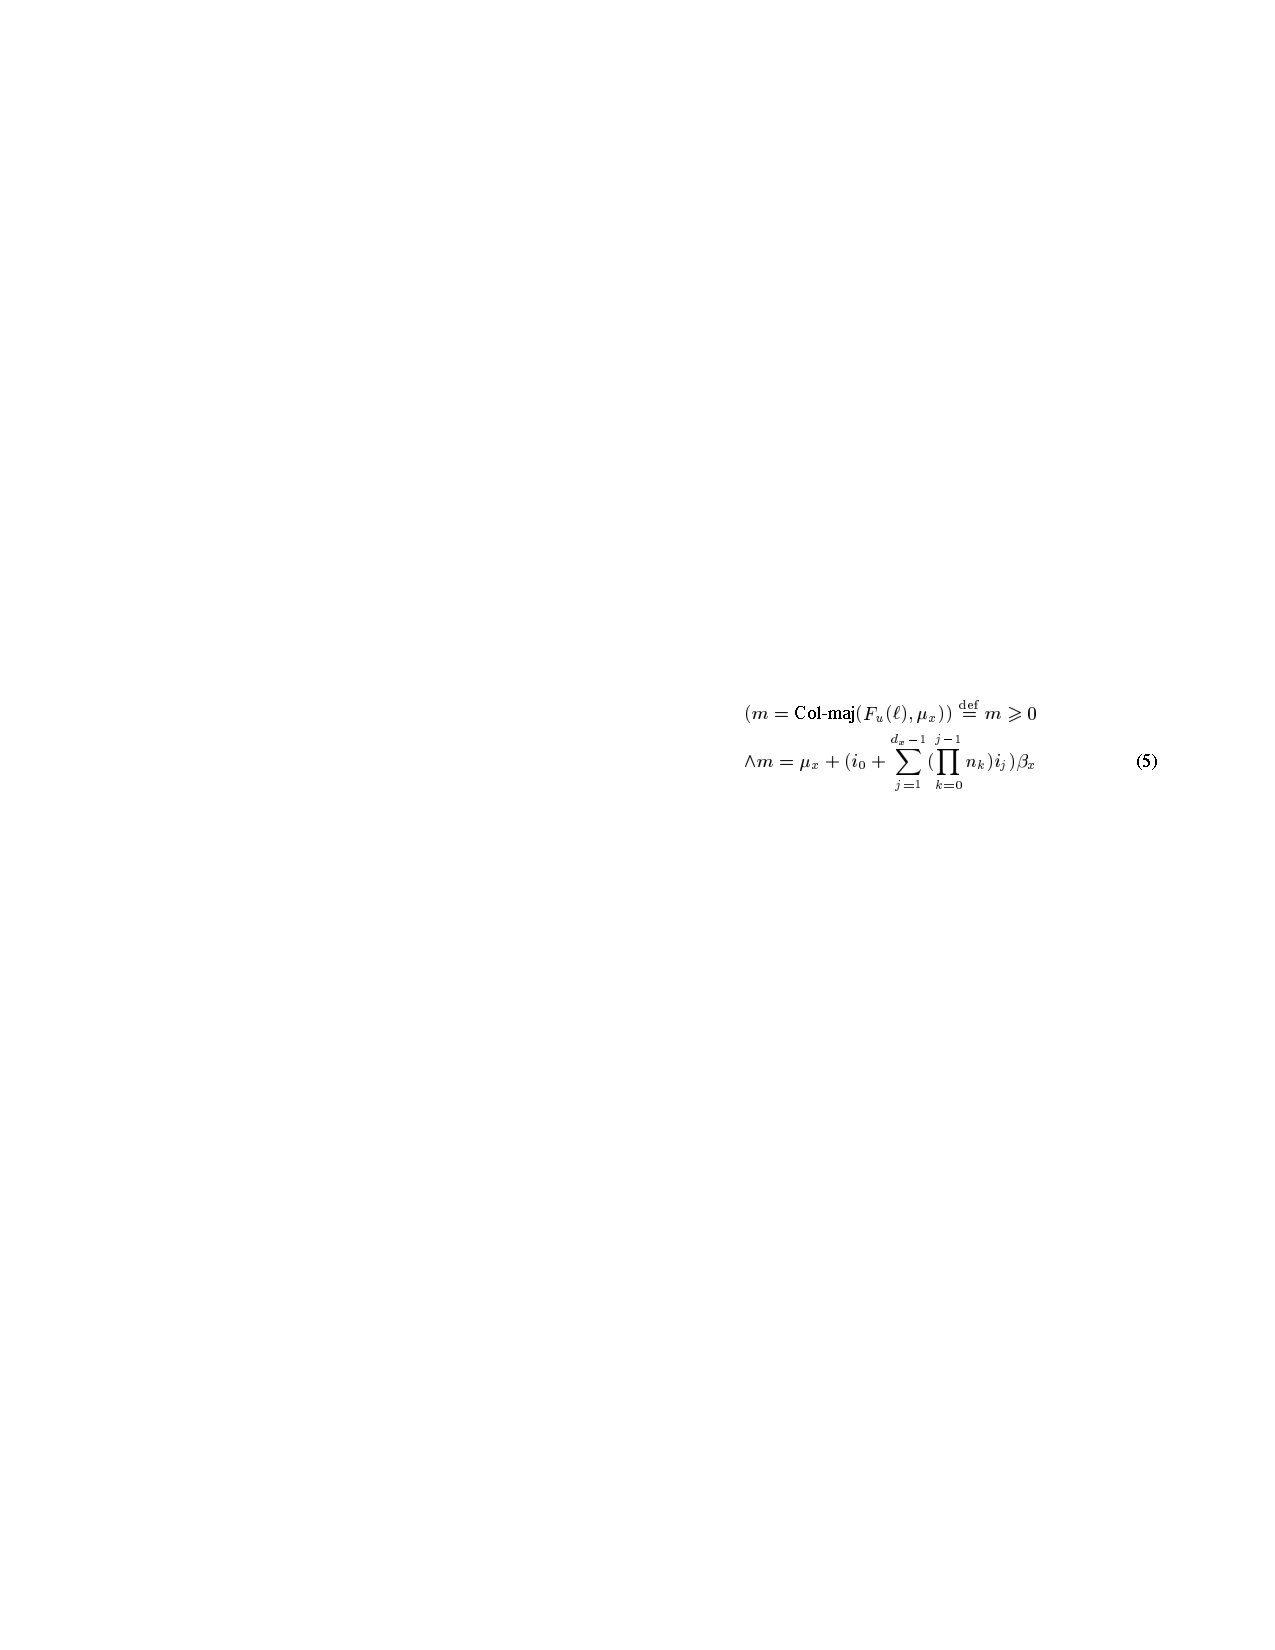
\includegraphics[scale=1.1]{eq5}
% % \label{fig:eq5}
% % \end{figure}
% Because we consider linear data layouts in the first place, we need a formulas to express raw and column major layouts.

\subsection{Cache Behavior}
For now, a direct-mapped cache is considered.

\subsubsection{Interior misses}
% \begin{figure}[H]
%         \centering
%         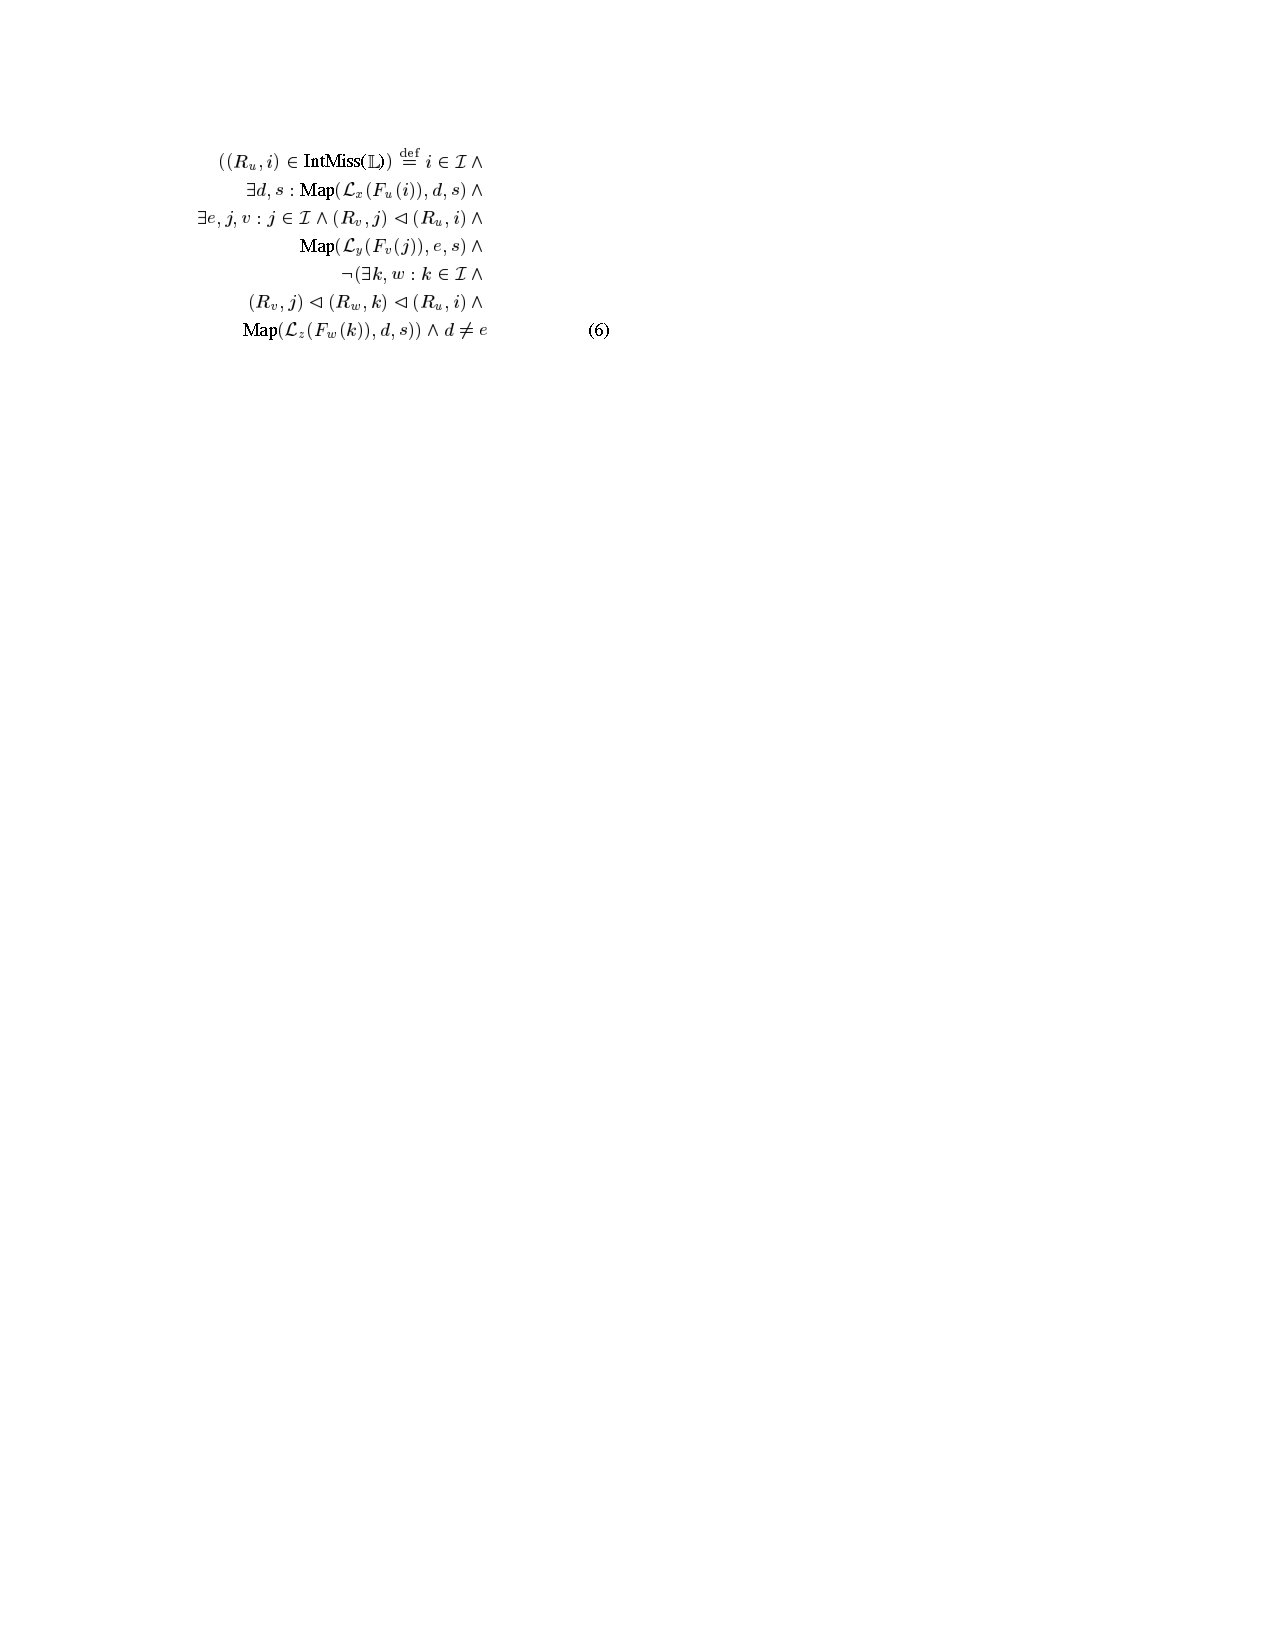
\includegraphics[scale=1.1]{eq6}
% \label{fig:eq6}
% \end{figure}
To determine if an access to a memory block $b$ results in an interior miss it is enough to now two things: (i) that there is an earlier access with a different memory block mapping to the same cache set; (ii) and that there is no access to $b$ between this earlier access and current access to $b$.
These properties can be expressed with formulas that we have seen.

\subsubsection{Boundary misses}
% \begin{figure}[H]
%         \centering
%         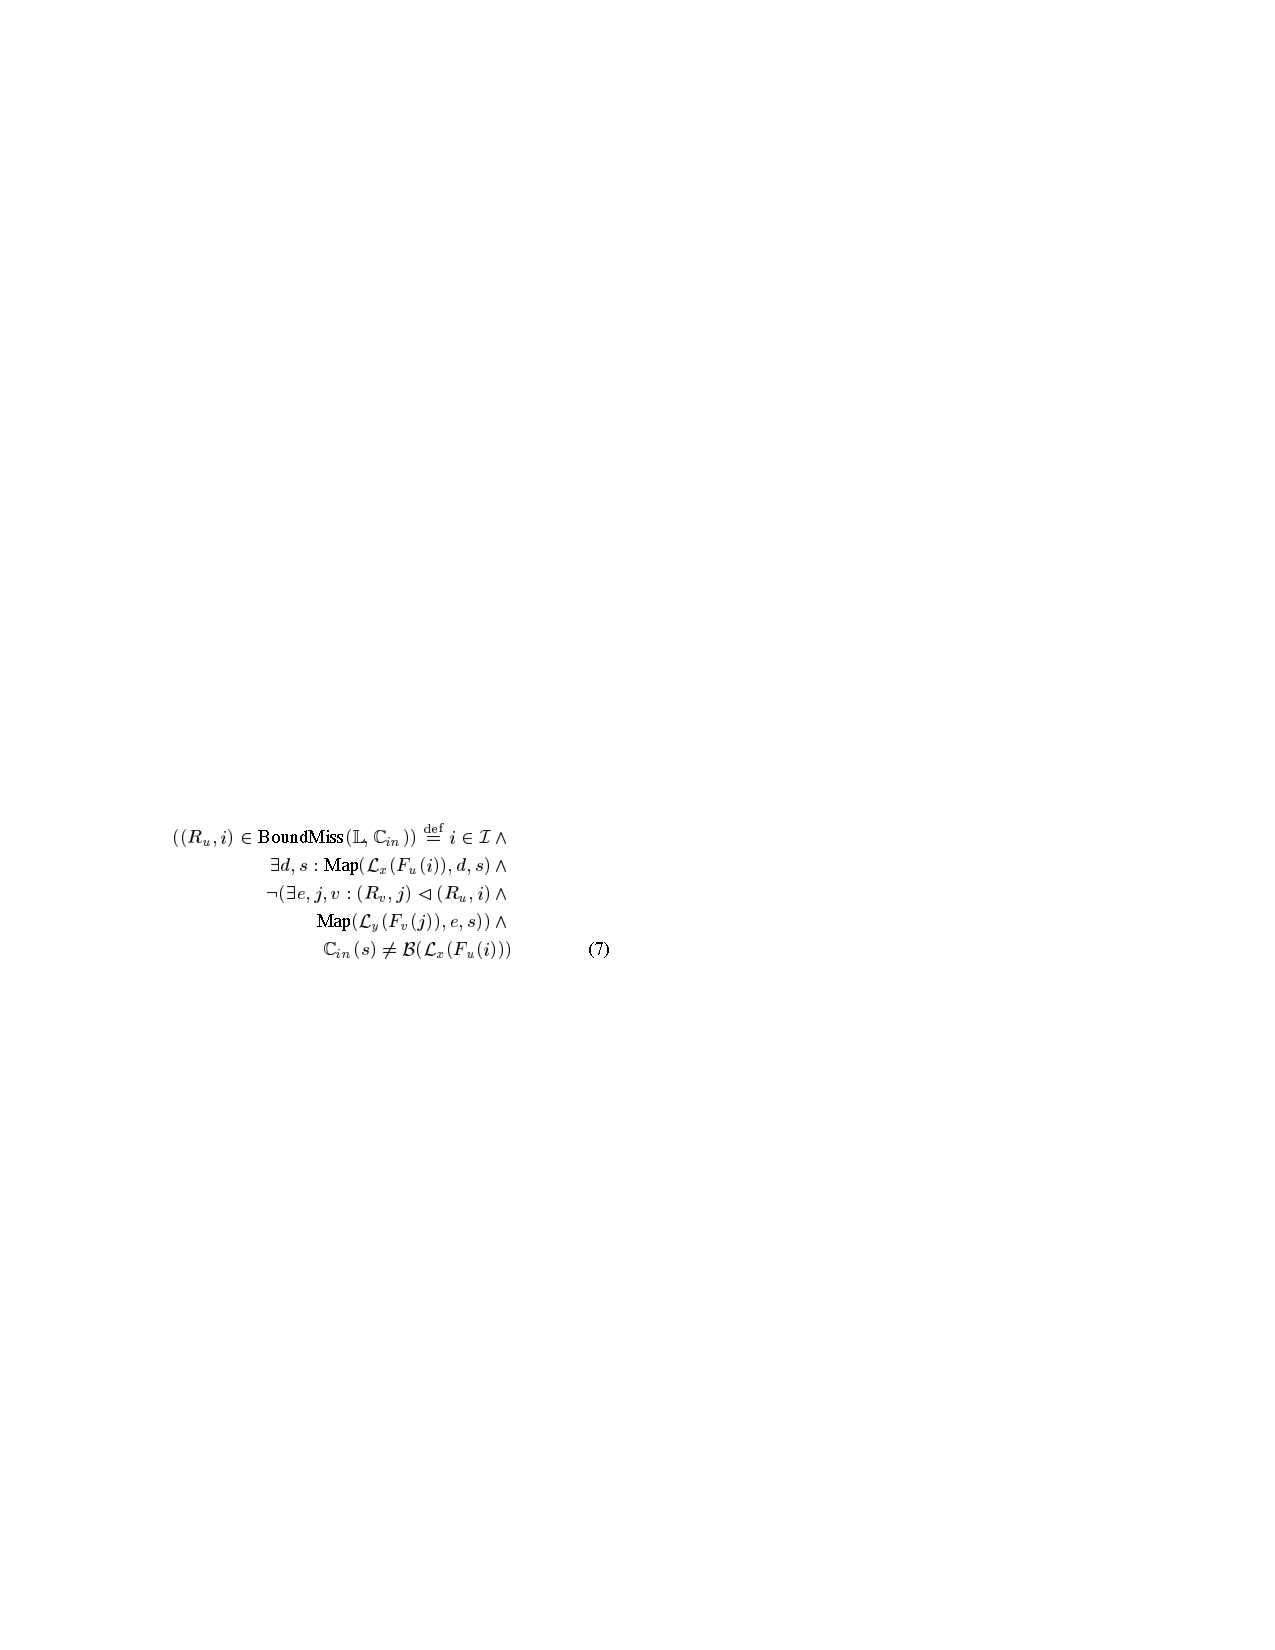
\includegraphics[scale=1.1]{eq7}
% \label{fig:eq7}
% \end{figure}
For boundary misses we are only interested in access that are the first to map to a cache set.
We can write the formula with previous formulas, but we also have to use the initial state of the cache to express that the memory block is not in the cache already.

\subsubsection{Cache state}
% \begin{figure}[H]
%         \centering
%         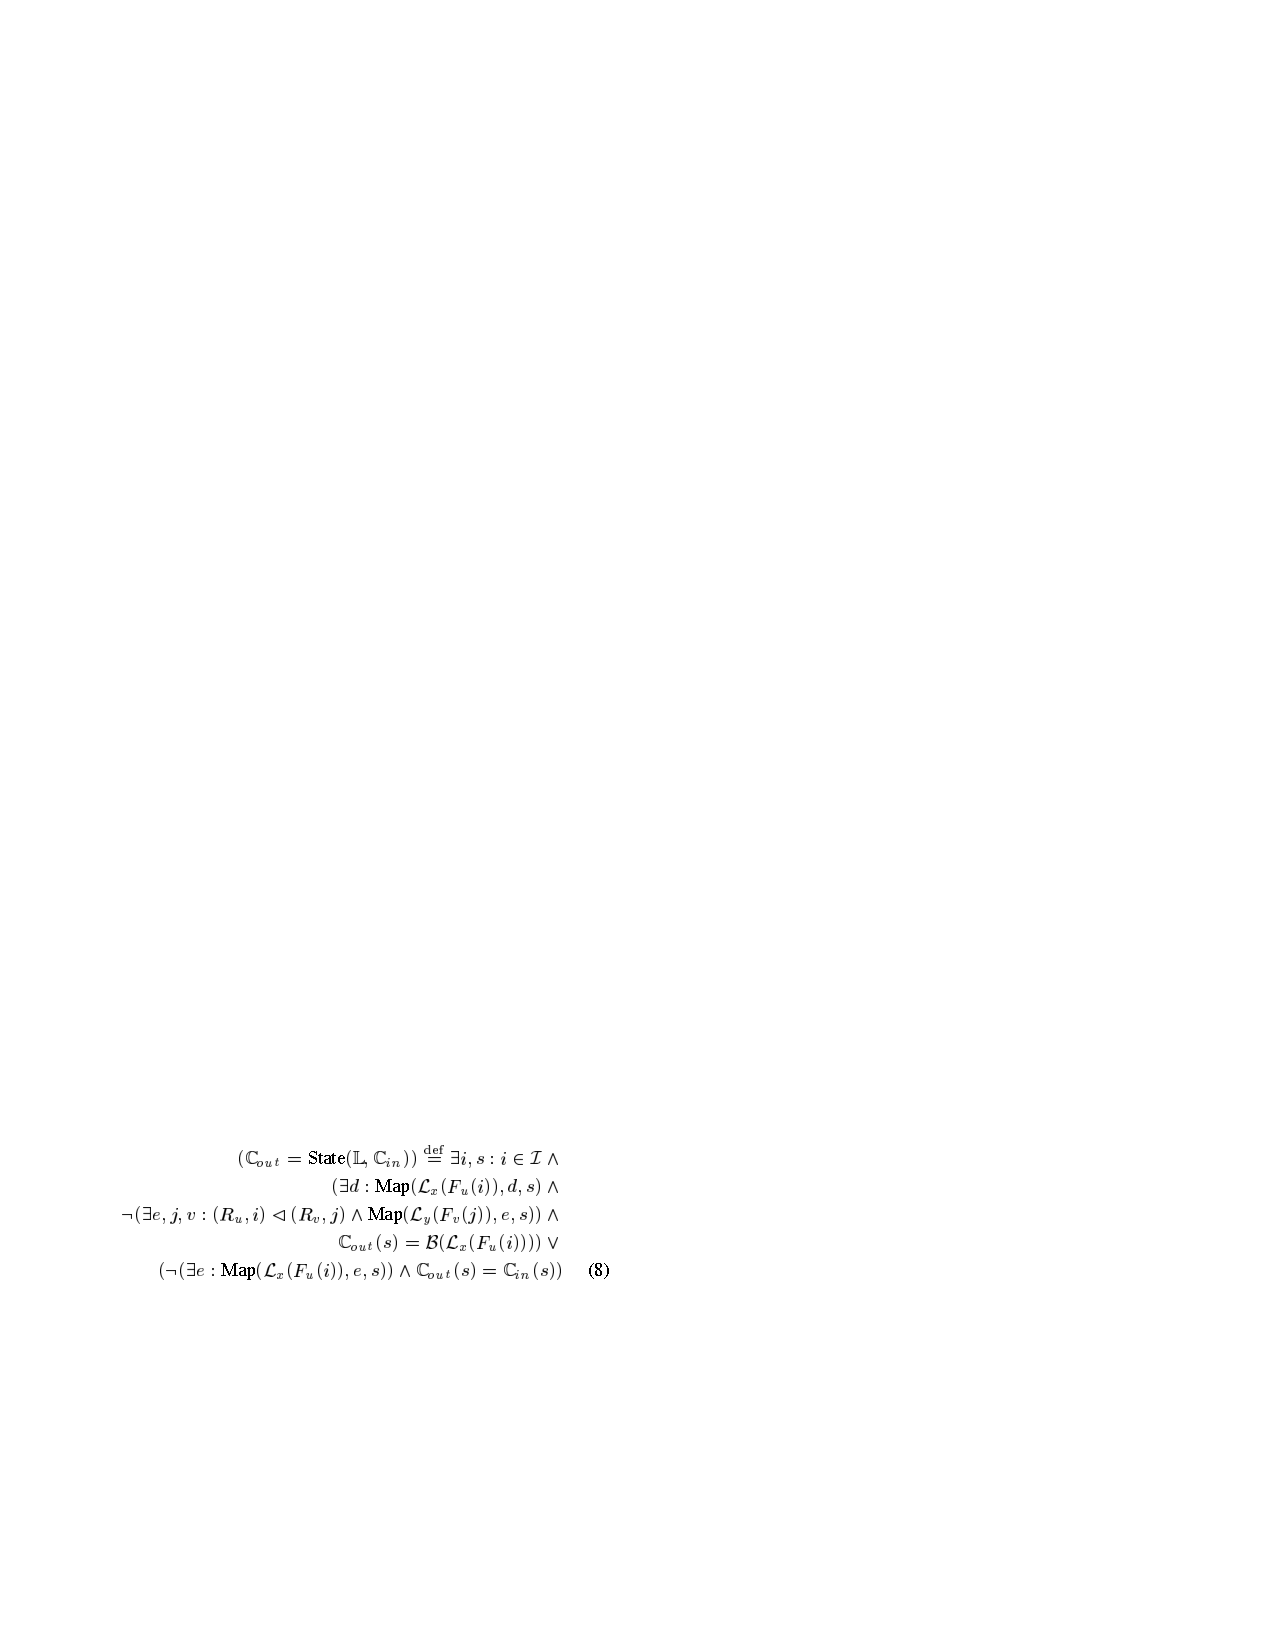
\includegraphics[scale=1.1]{eq8}
% \label{fig:eq8}
% \end{figure}
To have the final state of the cache we need to keep the memory block that have not been replaced.

% \subsection{Counting Cache Misses}

\subsection{Extensions}

\subsubsection{Imperfect loop nests}
Sometimes there are instructions outside the inner-most loop, which make loop nests \textit{imperfect}.
To handle these, they use a transformation~\cite{ahmed2001synthesizing} to move the problematic instructions in the inner-most with guards (i.e.\ \texttt{if} condition).
As the consequence they modified the formula of valid iteration point to include the guard's boolean condition.
% \begin{figure}[H]
%         \centering
%         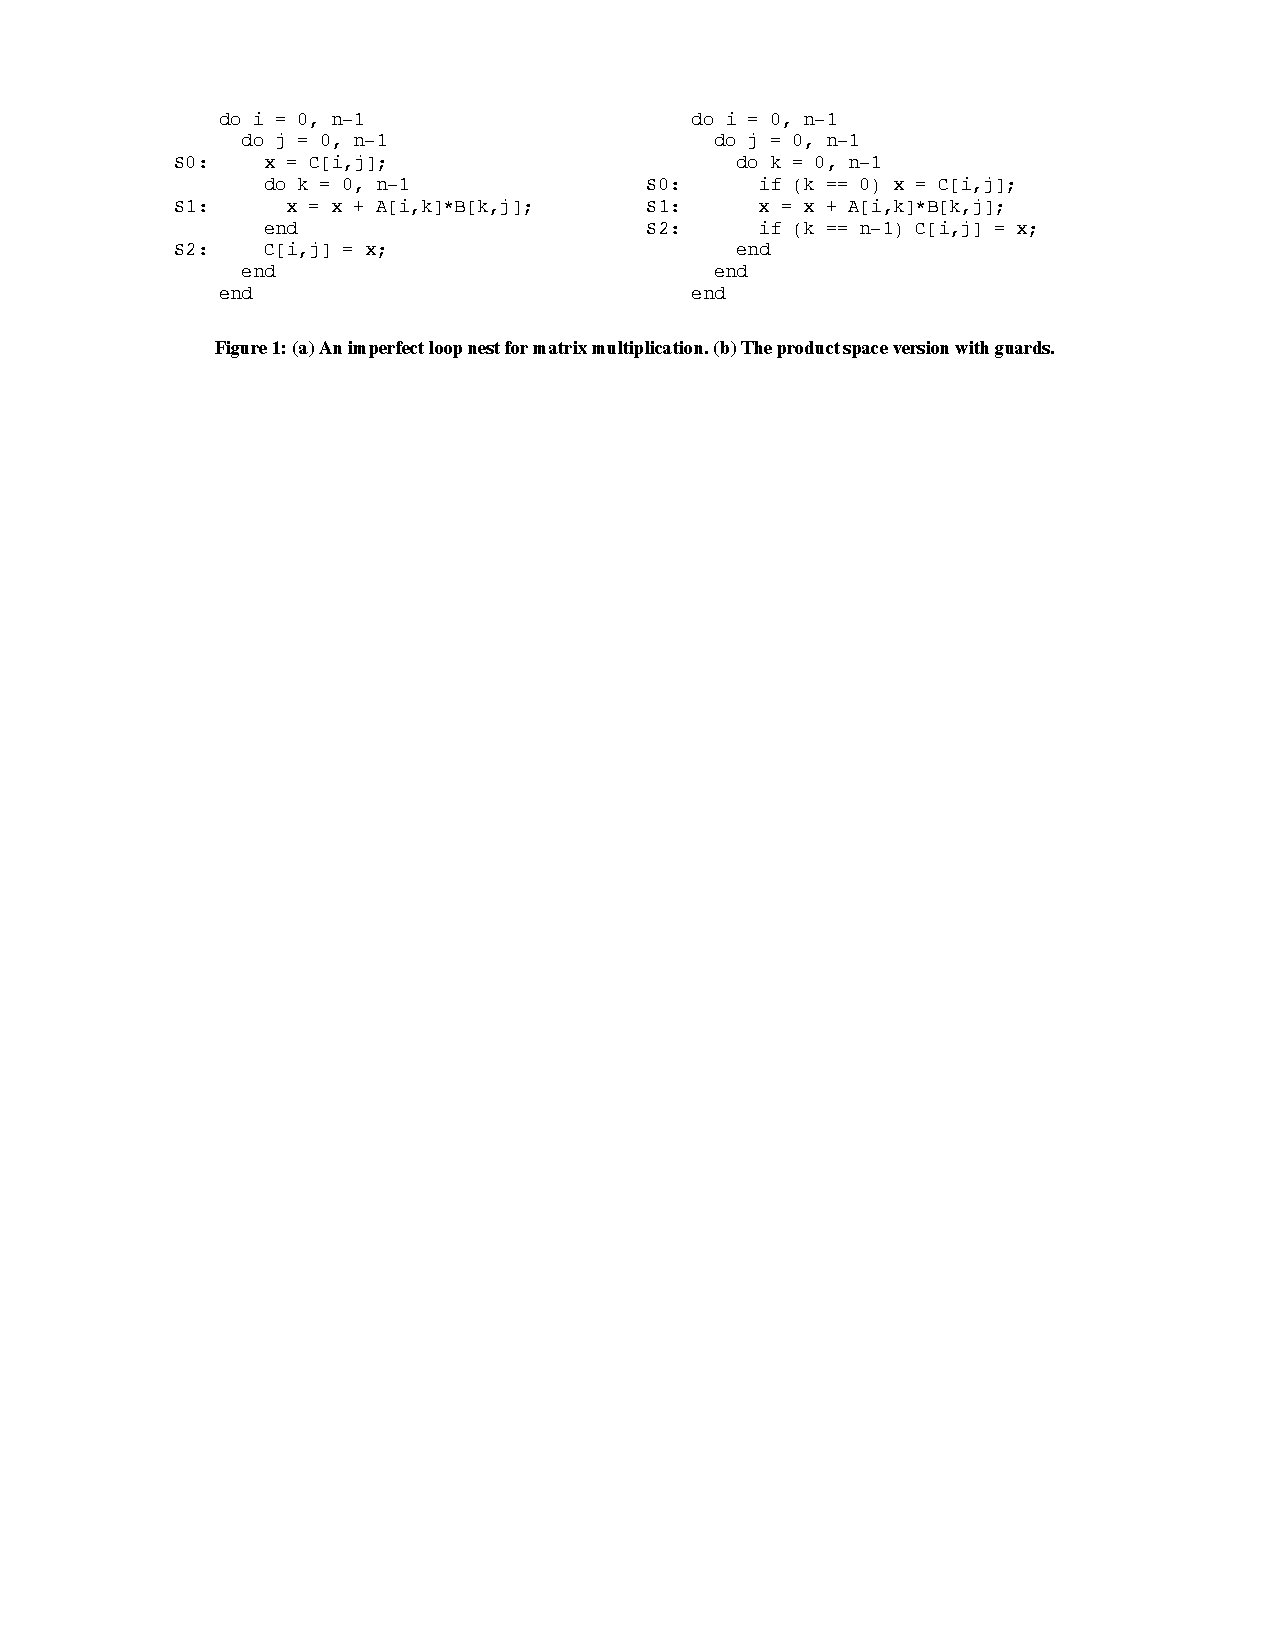
\includegraphics[trim={0 0.6cm 0 0}, clip]{figure1}
%         \caption{(a) An imperfect loop nest. (b) The product space version with guards.}
% \label{fig:imperfect}
% \end{figure}

\subsubsection{Associativity}
Defining interior misses with a A-way set-associative cache requires a longer formula as we can allow A different access before declaring a miss.
The downside is that the complexity of the formula increases with A to a point that only modest values of A can be handled.

\subsubsection{Non-linear data layouts}
To handle array layouts based on bit interleaving, memory addresses are expressed in binary to express the layouts in Presburger formulas.
Such fine grain grows the formula and thus has an impact in the overall complexity.


\section{Evaluation}
\label{eval}
To assess the correctness of their method they run it on different examples and compare the results with a cache simulation.
They run all possible loop permutations.
Examples include basic loop nests, imperfect loop nest, and non-linear arrays.

They find that the number of misses match, but that the classification differs.
This is because the cache simulation has a cold miss category which has no link with context as boundary misses do.


\section{Conclusion}
\label{critic}
The authors have developed a model that can exploit the regularity of loop nests to express the problem of counting cache misses in common mathematical formulas.
While it aims at replacing simulating, such model is still very much computationally expensive.
The authors propose as future work to mix both simulation and model-based computation to avoid polyhedral loop nests.

Assuming one memory access at a time without distinction between reads and writes seems reasonable.
Examples used in the evaluation were diverse enough to convince me of the correctness of the model.
While they assume a Least Recently Used replacement policy, I believe more complex policies could be modelled but I think it could make the A-way set-associativity complexity even worse.
In the same branch, they assume a two-level memory hierarchy, maybe the complexity would significantly increase with a third level.


\bibliographystyle{alpha}
\bibliography{biblio}

\end{document}
